\section{\MakeUppercase{Result and Analysis}}
\subsection{Dataset 1}
\subsubsection{Model Training}
The model is trained for 8 epochs taking batch size of 32. The training set consists of
8951 samples and testing set consists of 2238 samples. All these samples are generated
using random dataset generator.
\subsubsection{Loss vs Epoch Graph}
 \begin{figure}[H]
        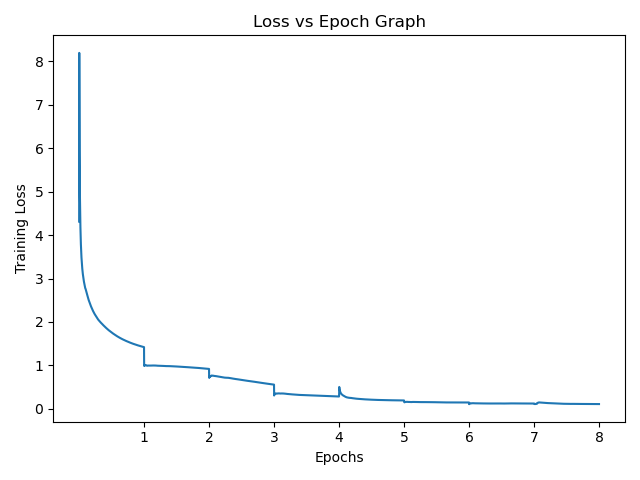
\includegraphics[scale=0.6]{images/Training Loss.png}
        \centering
        \caption{Loss vs Epoch graph for training time}
        \label{fig:lvsepoct}
    \end{figure}
     \begin{figure}[H]
        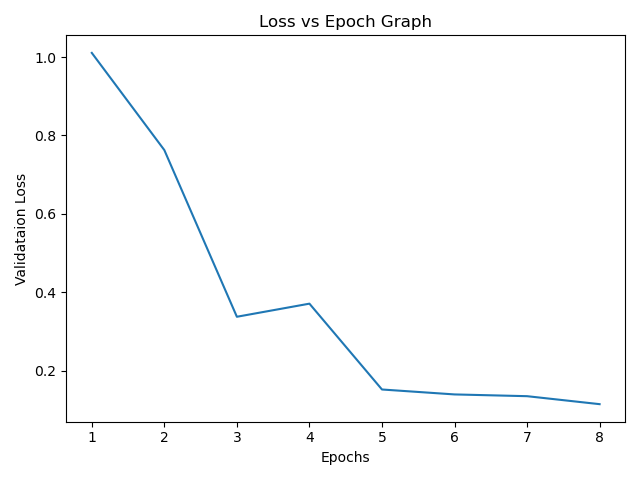
\includegraphics[scale=.6]{images/Validataion Loss.png}
        \centering
        \caption{Loss vs Epoch graph for validation time}
        \label{fig:lvsepochv}
    \end{figure}


        
Initially, the loss for the model is very high. In first epoch, the loss gradually decreased
and reached around 1.5. In the following epochs, the loss decreased steadily and
reached to 0.1 in the final epoch. The loss in validation set also remain comparable to
that of training set throughout the training which confirms model didn’t over fit for the
training data.
\subsubsection{Evaluation}
After training for 8 epochs, the model is evaluated on the test data. The BLEU and
ROUGE evaluation metrics are used to evaluate the model.

\textbf{BLEU Score}\\
The average BLEU score for n-grams 1, 2, 5 and 10 is as follows:
\begin{itemize}
    \item 1-grams BLEU Score: 0.9544114683715649
\item 2-grams BLEU Score: 0.9378854888760932
\item 5-grams BLEU Score: 0.8867411989388778
\item 10-grams BLEU Score: 0.7982317463855622
\end{itemize}
The above observation shows that good performance was achieved by the model on the given testing data. The average BLEU-1 score of 0.95 indicates that the generated DSL closely matches the reference DSL, suggesting that the model is effective at predicting the structure of short sequences. Although the BLEU score decreases as the n-gram size increases, a good performance is still maintained, indicating that the model excels at predicting short sequences. The BLEU-10 score of 0.79 further demonstrates that longer sequences were predicted accurately, showing the model’s ability to handle more complex and extended sequences.The individual BLEU-10 scores, sorted in order, were plotted in the graph. It can be observed that the BLEU-10 score is higher than 0.6 for most of the samples, reflecting consistent and reliable performance across a range of test cases. Additionally, numerous samples have BLEU scores above 0.9, supporting the conclusion that the model performed well across the testing data. This indicates that the model consistently generated high-quality results for both short and long sequences, confirming its reliability and effectiveness for the task.
 \begin{figure}[H]
        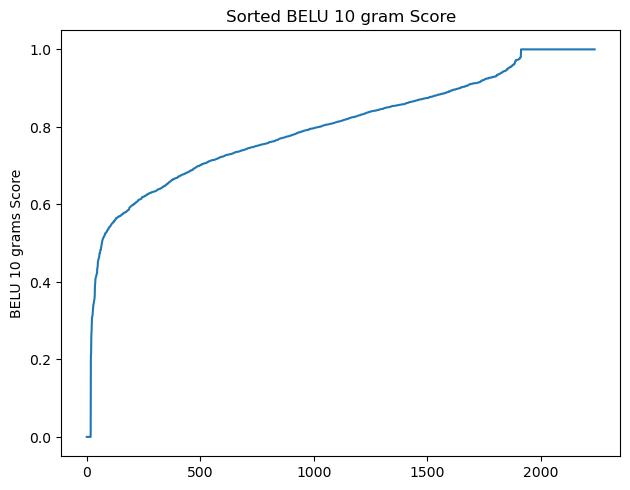
\includegraphics[scale=.8]{images/bleu in sorted order.png}
        \caption{BLEU-10 Scores in sorted order}
        \label{fig:bleu10}
    \end{figure}       
\textbf{ROUGE Score}\\
The average ROUGE Scores are tabulated below:
    Inserting table:
    \begin{table}[H]
        \caption{ROUGE Scores for test data}
        \label{tab:sample}
        \centering
        \begin{tabular}{|c|c|c|c|}
            \hline
            \textbf{Metric} & \textbf{Precision} & \textbf{Recall} &\textbf{F1-Score}\\
            \hline
            ROUGE-1 & 0.9481 & 0.9486 &0.9652 \\
            \hline
            ROUGE-5 & 0.7806&0.8112 & 0.7948 \\
            \hline
            ROUGE-L & 0.9428 & 0.9791 & 0.9598 \\
            \hline
        \end{tabular}
    \end{table}
    From above table, ROUGE-1 has high F1-score of 0.96. This indicates the predicted
tokens matches 96\% with the reference tokens. The ROUGE-5 F1-score is 0.79. It has
decreased drastically but it is still a good score. The high recall of 0.97 for ROUGE-L
indicates that the generated \gls{dsl} captures most of the longest common subsequences
from the reference. This indicates the generator maintains correct sequence and structure of \gls{dsl}. The graph below shows that the F1-score for almost all samples is
above 0.9 which is good performance.
 \begin{figure}[H]
        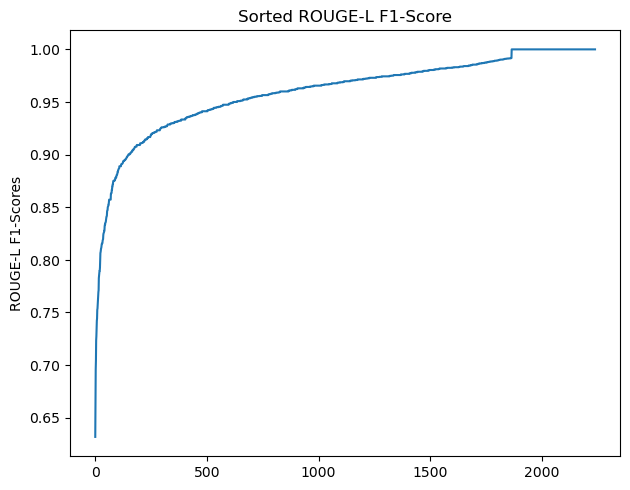
\includegraphics[scale=.8]{images/rouge-L F1-scores in sorted order.png}
        \centering
        \caption{ROUGE-L F1-Scores in sorted order}
        \label{fig:rouge-l-F1 score}
    \end{figure}
\subsection{Dataset 2}
By improving the dataset generation process the new sets of dataset comprising of about 19000 images is generated. The new samples of elements are collected and data is generated.  13510 images were used for training and 5790 images were used for validation purpose. The three different models were trained for the given data. The 100 hand drawn images were used to evaluate the performance of all three models. The associated dsl code for the hand drawn images were provided manually by human evaluation based on the rule.
\subsubsection{Model 1(Compact Convolutional Transformer Encoder with Transformer Decoder)}
\begin{figure}[H]
    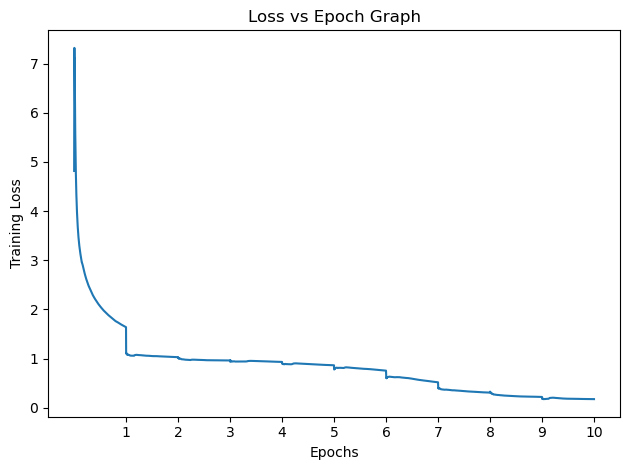
\includegraphics[scale=.8]{images/tl1.png}
    \centering
    \caption{Training loss vs Epoch graph(Model 1)}
    \label{fig:cctewtd}
\end{figure}
\begin{figure}[H]
    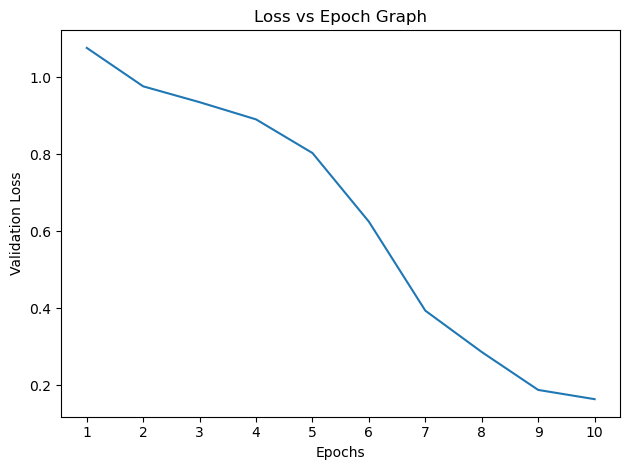
\includegraphics[scale=.8]{images/vl1.png}
    \centering
    \caption{Validation loss vs Epoch graph(Model 1)}
    \label{fig:cctewtdv}
\end{figure}
Initially, the loss for the model is very high. The model get familiar with the nature of the data and associated output in the first epoch and the loss decreased rapidly in the first epoch. During next 9 epochs, the loss gradually decreased from 1 to near 0. The decreasing nature of the graph indicates the model is learning the nature of data quiet well. The loss has gradually decreased in both training and validation. The loss decreased from 4.81 to 0.17 at the end of 10th epoch. The masked accuracy of 0.93 was achieved for training data and same for the validation data.\\
\\
\textbf{Evaluation}\\
The ROUGE and BlEU metric is used to evaluate the performance of the model in 100 hand drawn images.

\textbf{BLEU Score}\\
The average BLEU score for n-grams 1,2,5 and 10 is follows:
\begin{itemize}
    \item 1-grams BLEU Score: 0.7471271688303959
    \item 2-grams BLEU Score: 0.6580029789136941
    \item 5-grams BLEU Score:  0.42442962967602715
    \item 10-grams BLEU Score: 0.30114337436735683
\end{itemize}
\textbf{ROUGE Score}\\
The average rouge score obtained for the test data are tabulated below.
\begin{table}[H]
    \caption{ROUGE Scores for test data (model1)}
    \label{tab:sampl}
    \centering
    \begin{tabular}{|c|c|c|c|}
        \hline
        \textbf{Metric} & \textbf{Precision} & \textbf{Recall} &\textbf{F1-Score}\\
        \hline
        ROUGE-1 & 0.7124 & 0.7768 &0.7385 \\
        \hline
        ROUGE-5 & 0.4218&0.4732 & 0.4467 \\
        \hline
        ROUGE-L & 0.6261 & 0.6823 & 0.6487 \\
        \hline
    \end{tabular}
\end{table}
% From above table, ROUGE-1 recall is 0.7768 that indicates that 77.6\% predicted tokens matched reference tokens of the data.  While considering 5 tokens at a time, the score reached 0.47. For the longest subsequence, the recall score obtained is 68\%. The graph consisting of ROUGE L scores in the sorted order is presented below:
\begin{figure}[H]
    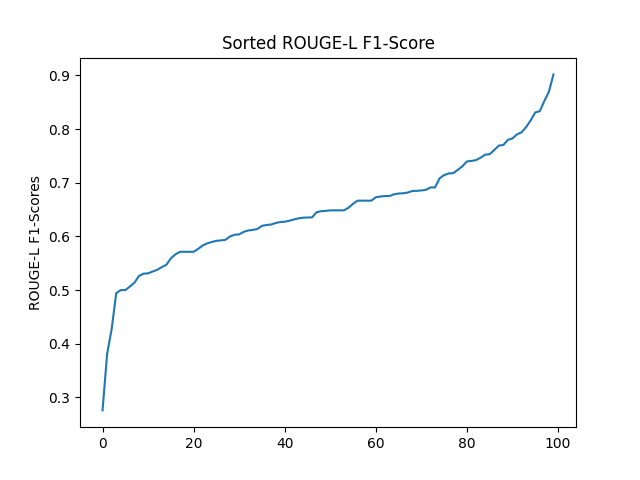
\includegraphics[scale=.8]{images/sr1.png}
    \caption{Sorted Rouge-L F1-Score(Model 1)}
    \label{fig:lf11}
\end{figure}
It is seen that ROUGE-L score is more than 0.5 for most of data leaving 3 images. The most of the data have score between 0.5 and 0.7. There are also many number of images with score above 0.7. The highest score is 0.9019 and the lowest score is 0.2758. The best and worst case test data is shown below:
\begin{figure}[H]
    \centering
    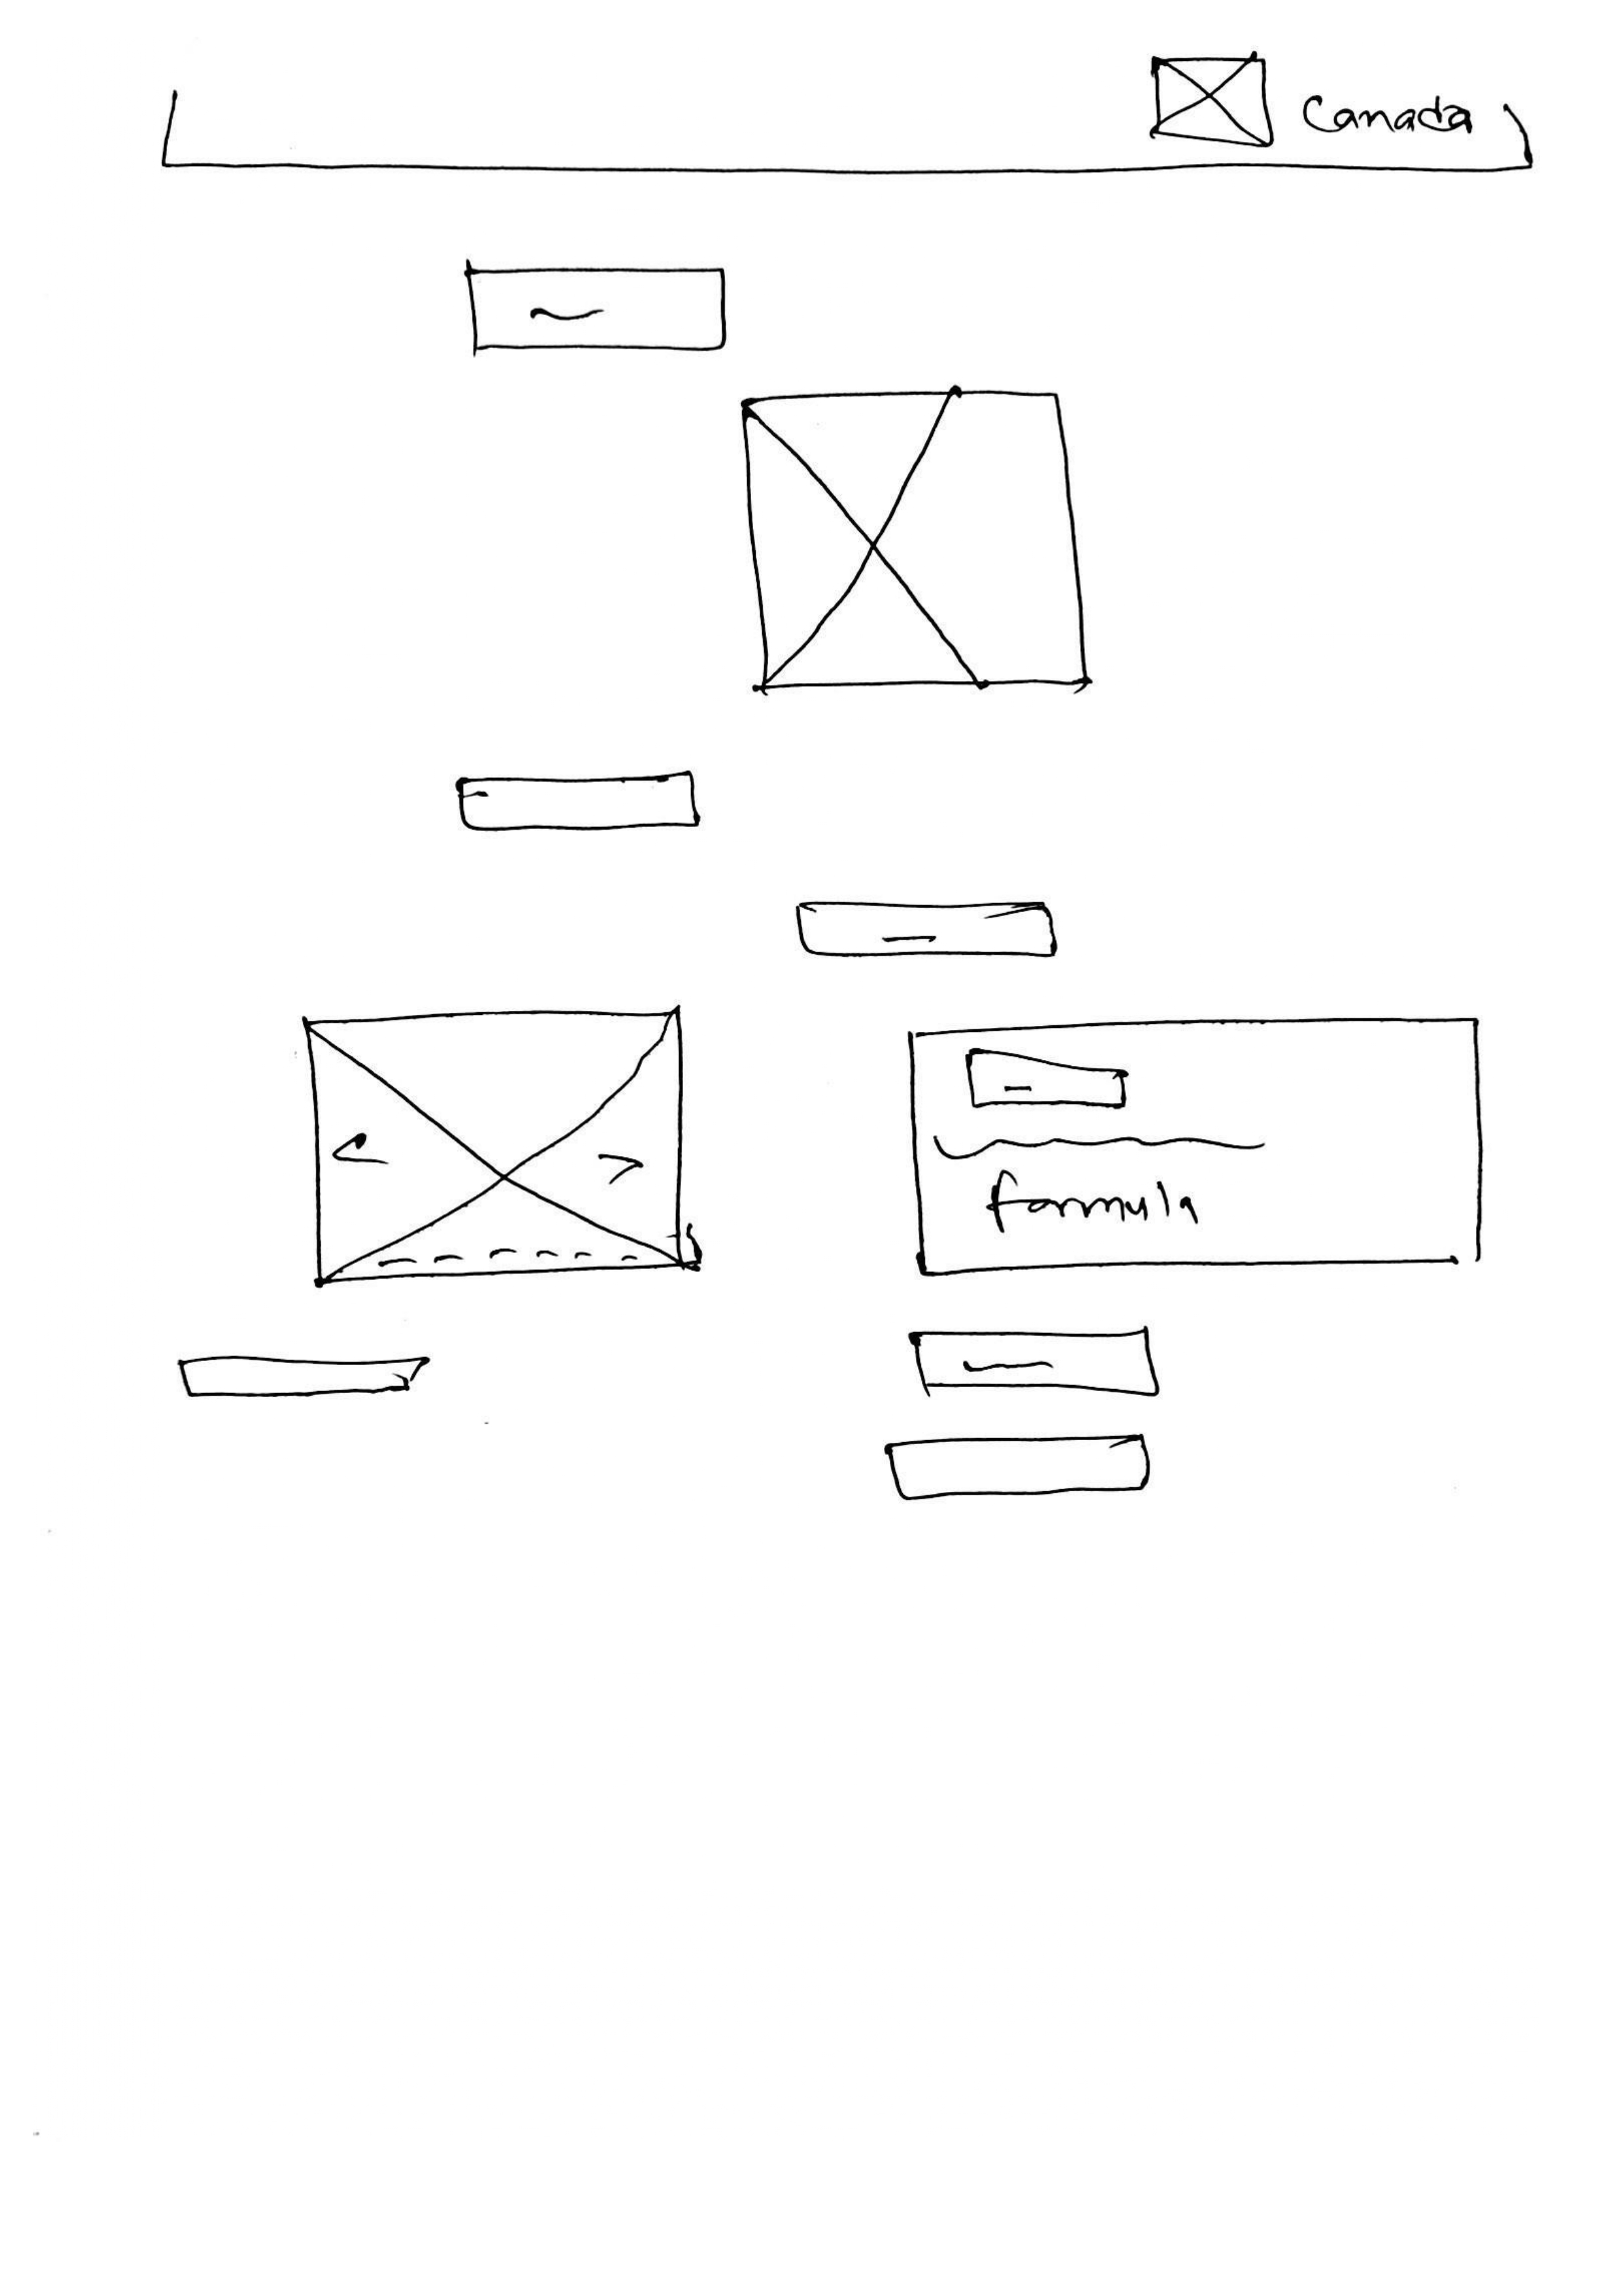
\includegraphics[scale=.35, trim=230 300 190 10]{images/m11.jpg}
    \caption{Input Image(ROUGE-L score 0.901)}
    \label{fig:m11}
\end{figure}

\begin{figure}[H]
    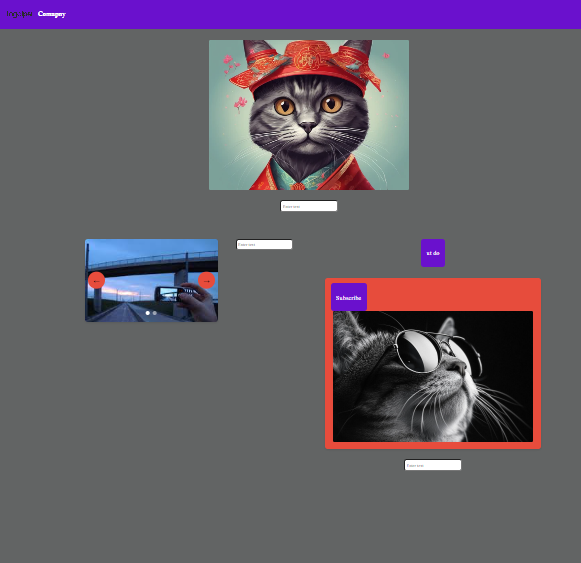
\includegraphics[scale=.5]{images/m101.png}
    \centering
    \caption{Output(ROUGE-L Score 0.901)}
    \label{fig:m12}
\end{figure}

\begin{figure}[H]
    \centering
    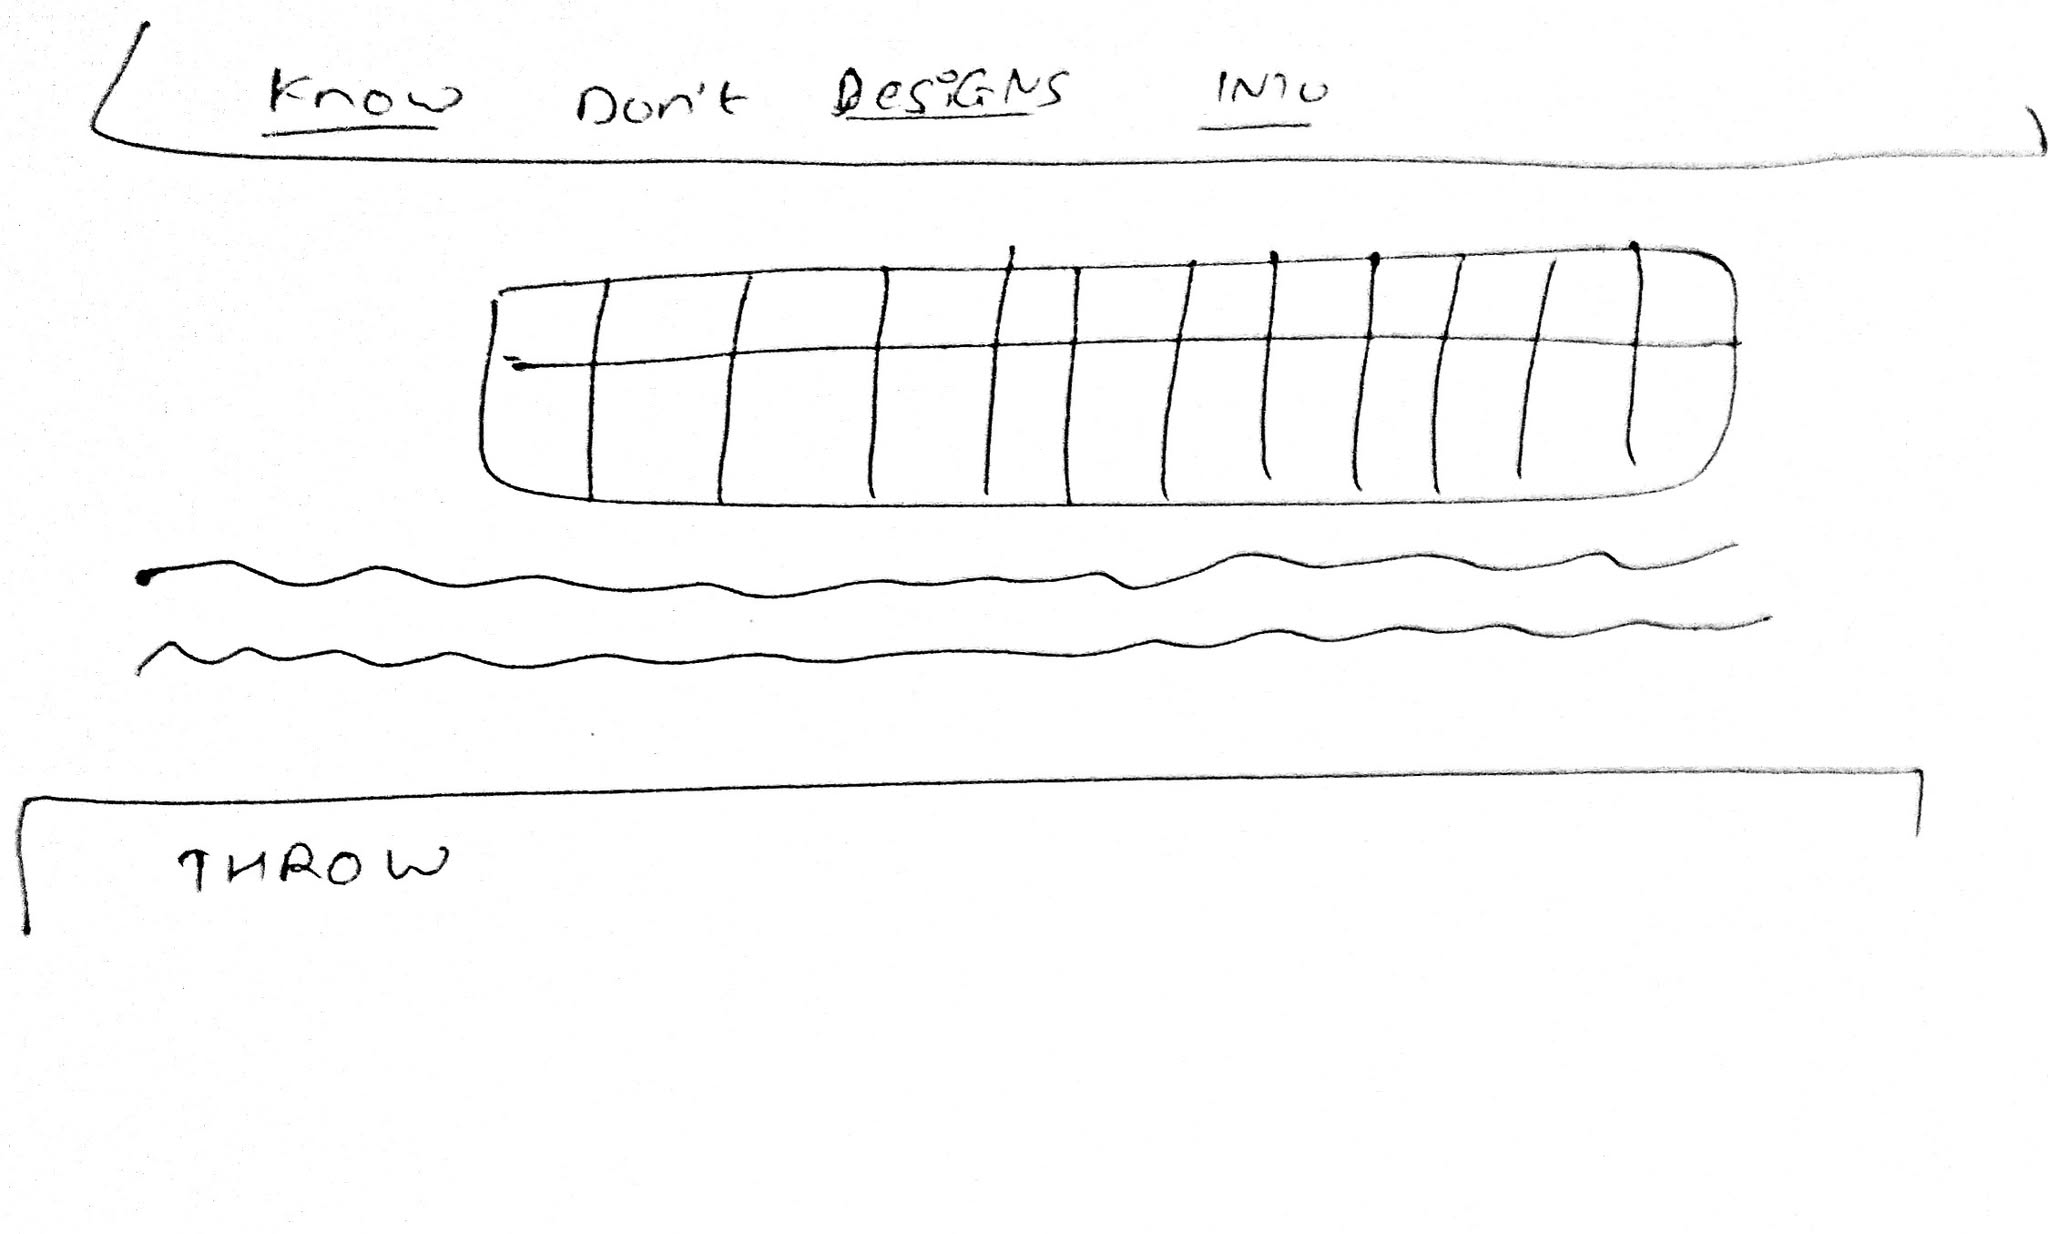
\includegraphics[scale=.1]{images/n1.jpg}
    \caption{Input Image(ROUGE-L Score 0.2758)}
    \label{fig:m13}
\end{figure}

\begin{figure}[H]
    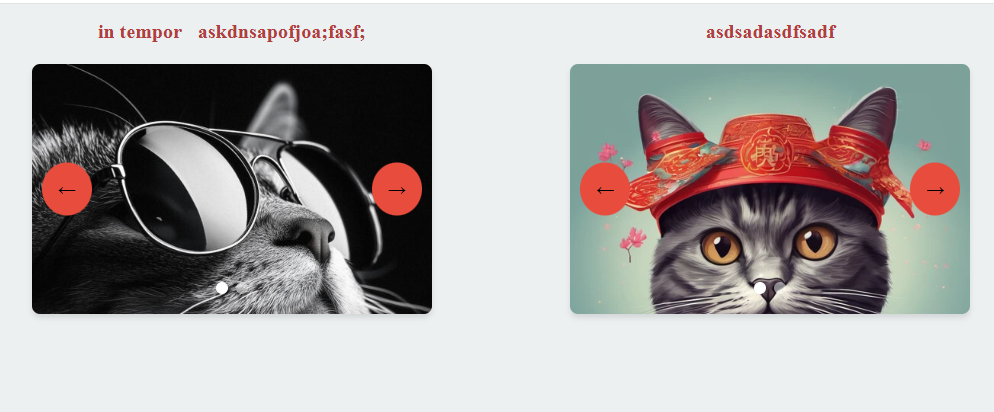
\includegraphics[scale=.35]{images/m1o2.png}
    \caption{Output(ROUGE-L score 0.2758)}
    \label{fig:m14}
\end{figure}





\subsubsection{Model 2(Vision Transformer Encoder with Transformer Decoder)}
\begin{figure}[H]
    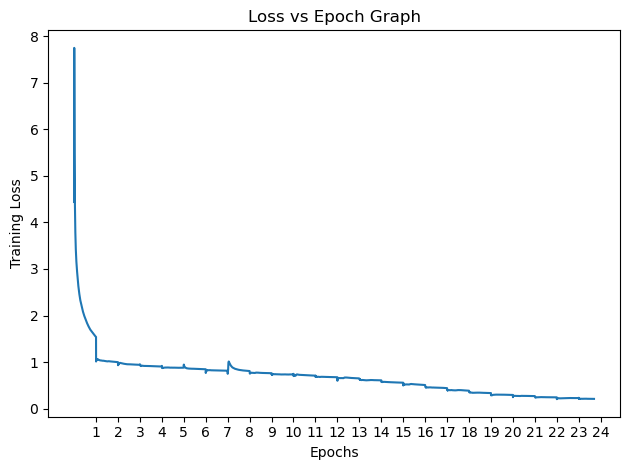
\includegraphics[scale=.8]{images/tl2.png}
    \caption{Training Loss Vs Epoch(Model 2)}
    \label{fig:tl2}
\end{figure}
\begin{figure}[H]
    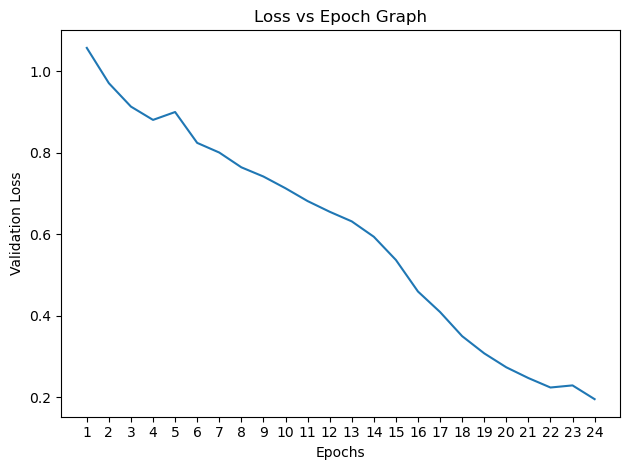
\includegraphics[scale=.8]{images/vl2.png}
    \caption{Validation Loss vs Epoch(Model 2)}
    \label{fig:vl2}
\end{figure}
The patch of size 16x16 is extracted from the image of size (848,608). The loss of the training data decreased rapidly from 7.23 to 1.54 in the first epoch of training. It indicates the model was able to learn about the data during the training. In the subsequent iterations, the loss of both training and validation data decreased gradually. The rate at which the loss decreased is found to be slower than for model 1. The training loss of 0.2 was reached after training for 24 epochs. The training was stopped as the loss start to increase. The masked accuracy of 0.91 was reached at the end of the training.

\textbf{Evaluation}\\
    The ROUGE and BlEU metric is used to evaluate the performance of the model in 100 hand drawn images.

\textbf{BLEU Score}\\
The average BLEU score for n-grams 1,2,5 and 10 is follows:
\begin{itemize}
    \item 1-grams BLEU Score: 0.6798317754323199
    \item 2-grams BLEU Score: 0.5806978773972931
    \item 5-grams BLEU Score:  0.3387053560764535
    \item 10-grams BLEU Score: 0.25798579488789025
\end{itemize}

\textbf{ROUGE Score}\\
The average rouge score obtained for the test data are tabulated below.
\begin{table}[H]
    \caption{ROUGE Scores for test data(Model 2)}
    \label{tab:samp}
    \centering
    \begin{tabular}{|c|c|c|c|}
        \hline
        \textbf{Metric} & \textbf{Precision} & \textbf{Recall} &\textbf{F1-Score}\\
        \hline
        ROUGE-1 & 0.6329 & 0.7560 &0.6749 \\
        \hline
        ROUGE-5 & 0.3842 & 0.4589 & 0.4091 \\
        \hline
        ROUGE-L & 0.5244 & 0.6256 & 0.5583 \\
        \hline
    \end{tabular}
\end{table}
From above table, ROUGE-1 recall is 0.756 that indicates that 75\% predicted tokens matched reference tokens of the data.  While considering 5 tokens at a time, the score reached 0.45. For the longest subsequence, the recall score obtained is 62\%. The graph consisting of ROUGE L scores in the sorted order is presented below:
\begin{figure}[H]
    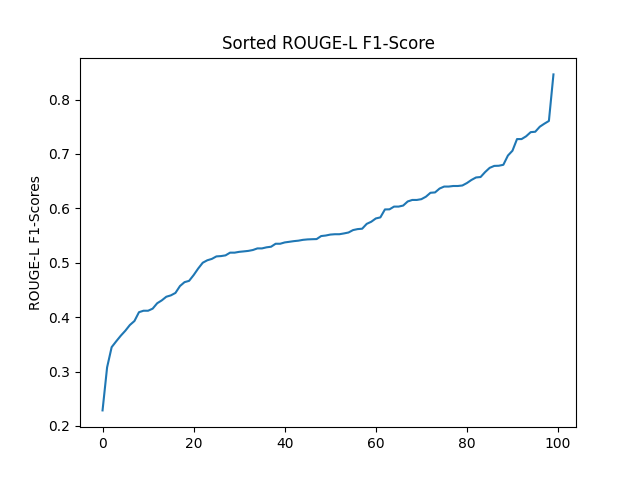
\includegraphics[scale=.8]{images/sr2.png}
    \caption{Sorted ROUGE-L F1-Scores in sorted order(Model 2)}
    \label{fig:srlf}
\end{figure}
It is seen that ROUGE-L score is more than 0.5 for most of data. The most of the data have score between 0.5 and 0.7. The few samples have the score above the 0.7. The minimum score is 0.22 and the maximum score obtained is 0.845. The best and worst case test data is shown below:
\begin{figure}[H]
    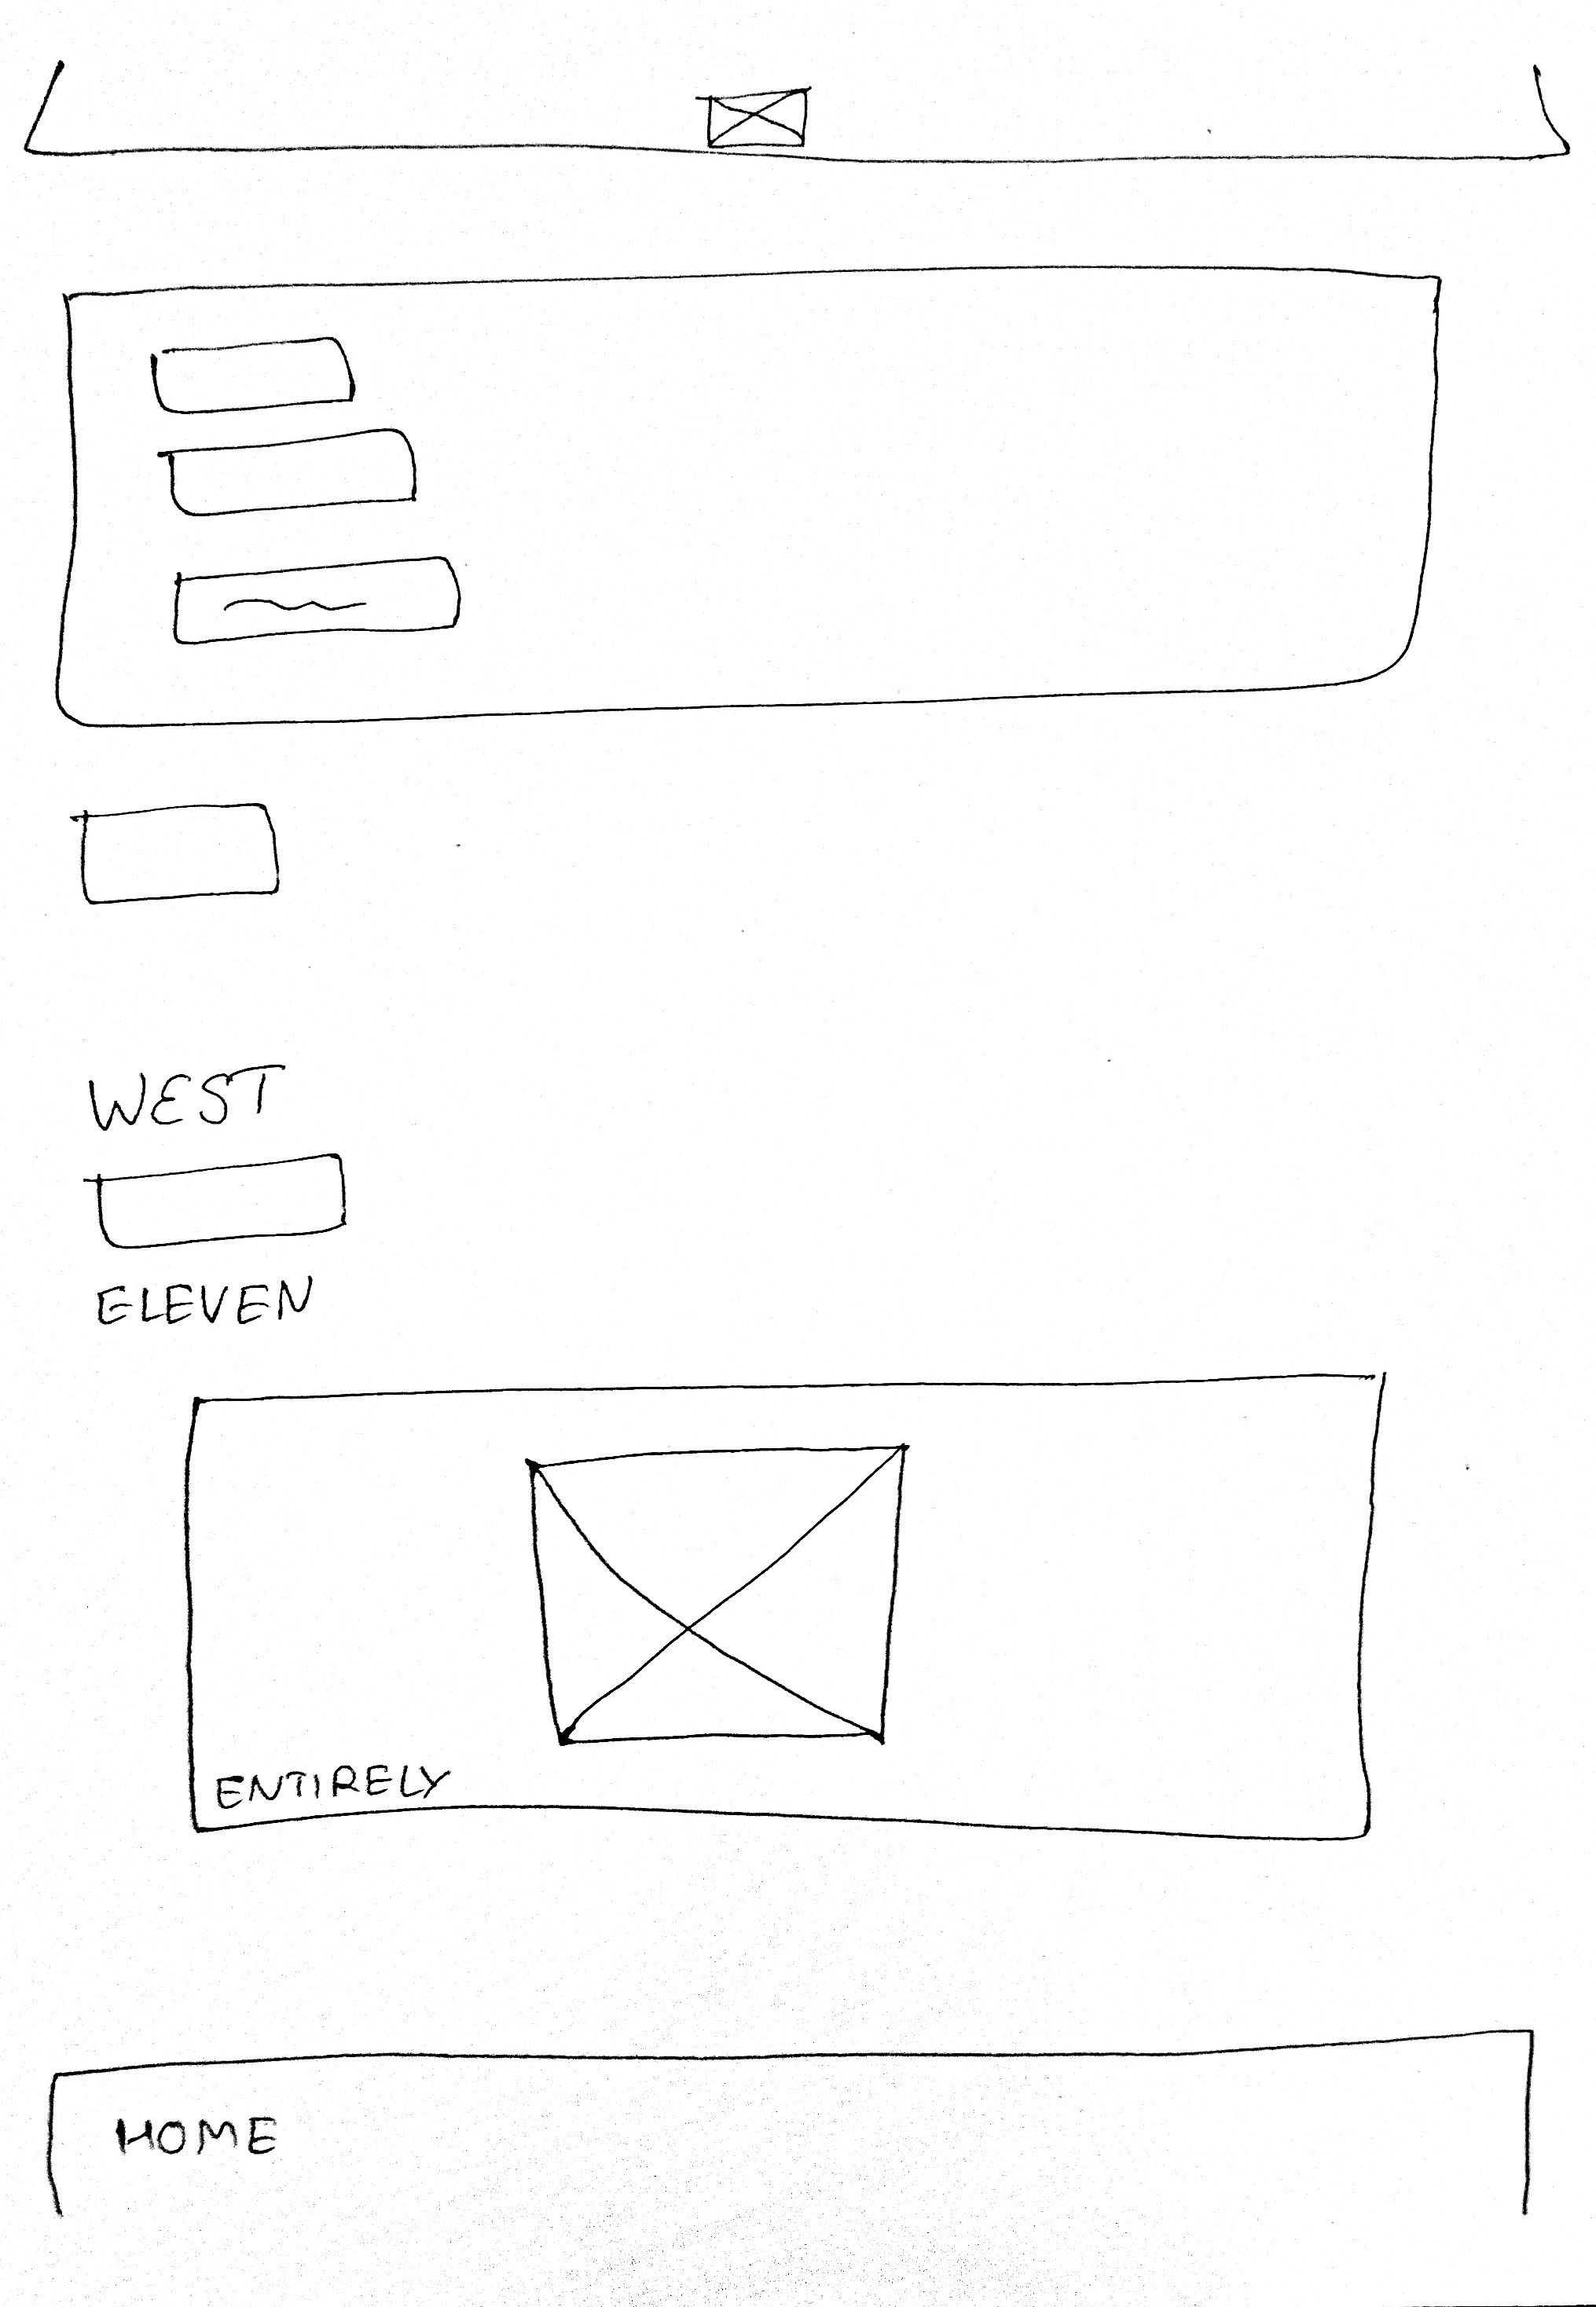
\includegraphics[scale=.1]{images/m22.jpg}
    \centering
    \caption{Input Image(ROUGE-L score 0.845)}
    \label{fig:m22}
\end{figure}

\begin{figure}[H]
    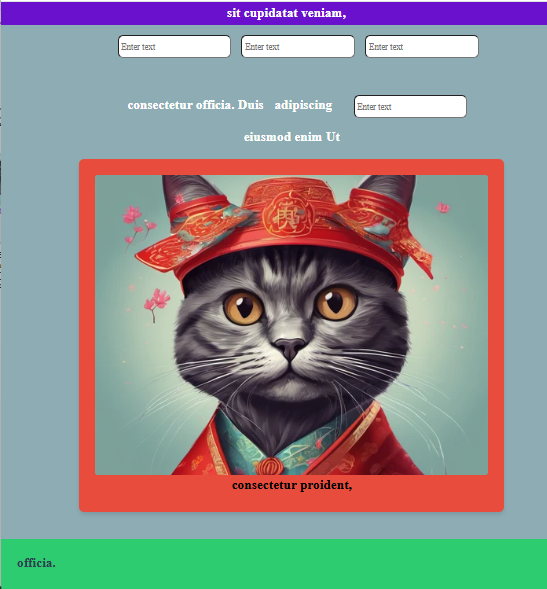
\includegraphics[scale=.8]{images/m2o3.png}
    \centering
    \caption{Output(ROUGE-L score 0.845) }
    \label{fig:m21}
\end{figure}

\begin{figure}[H]
    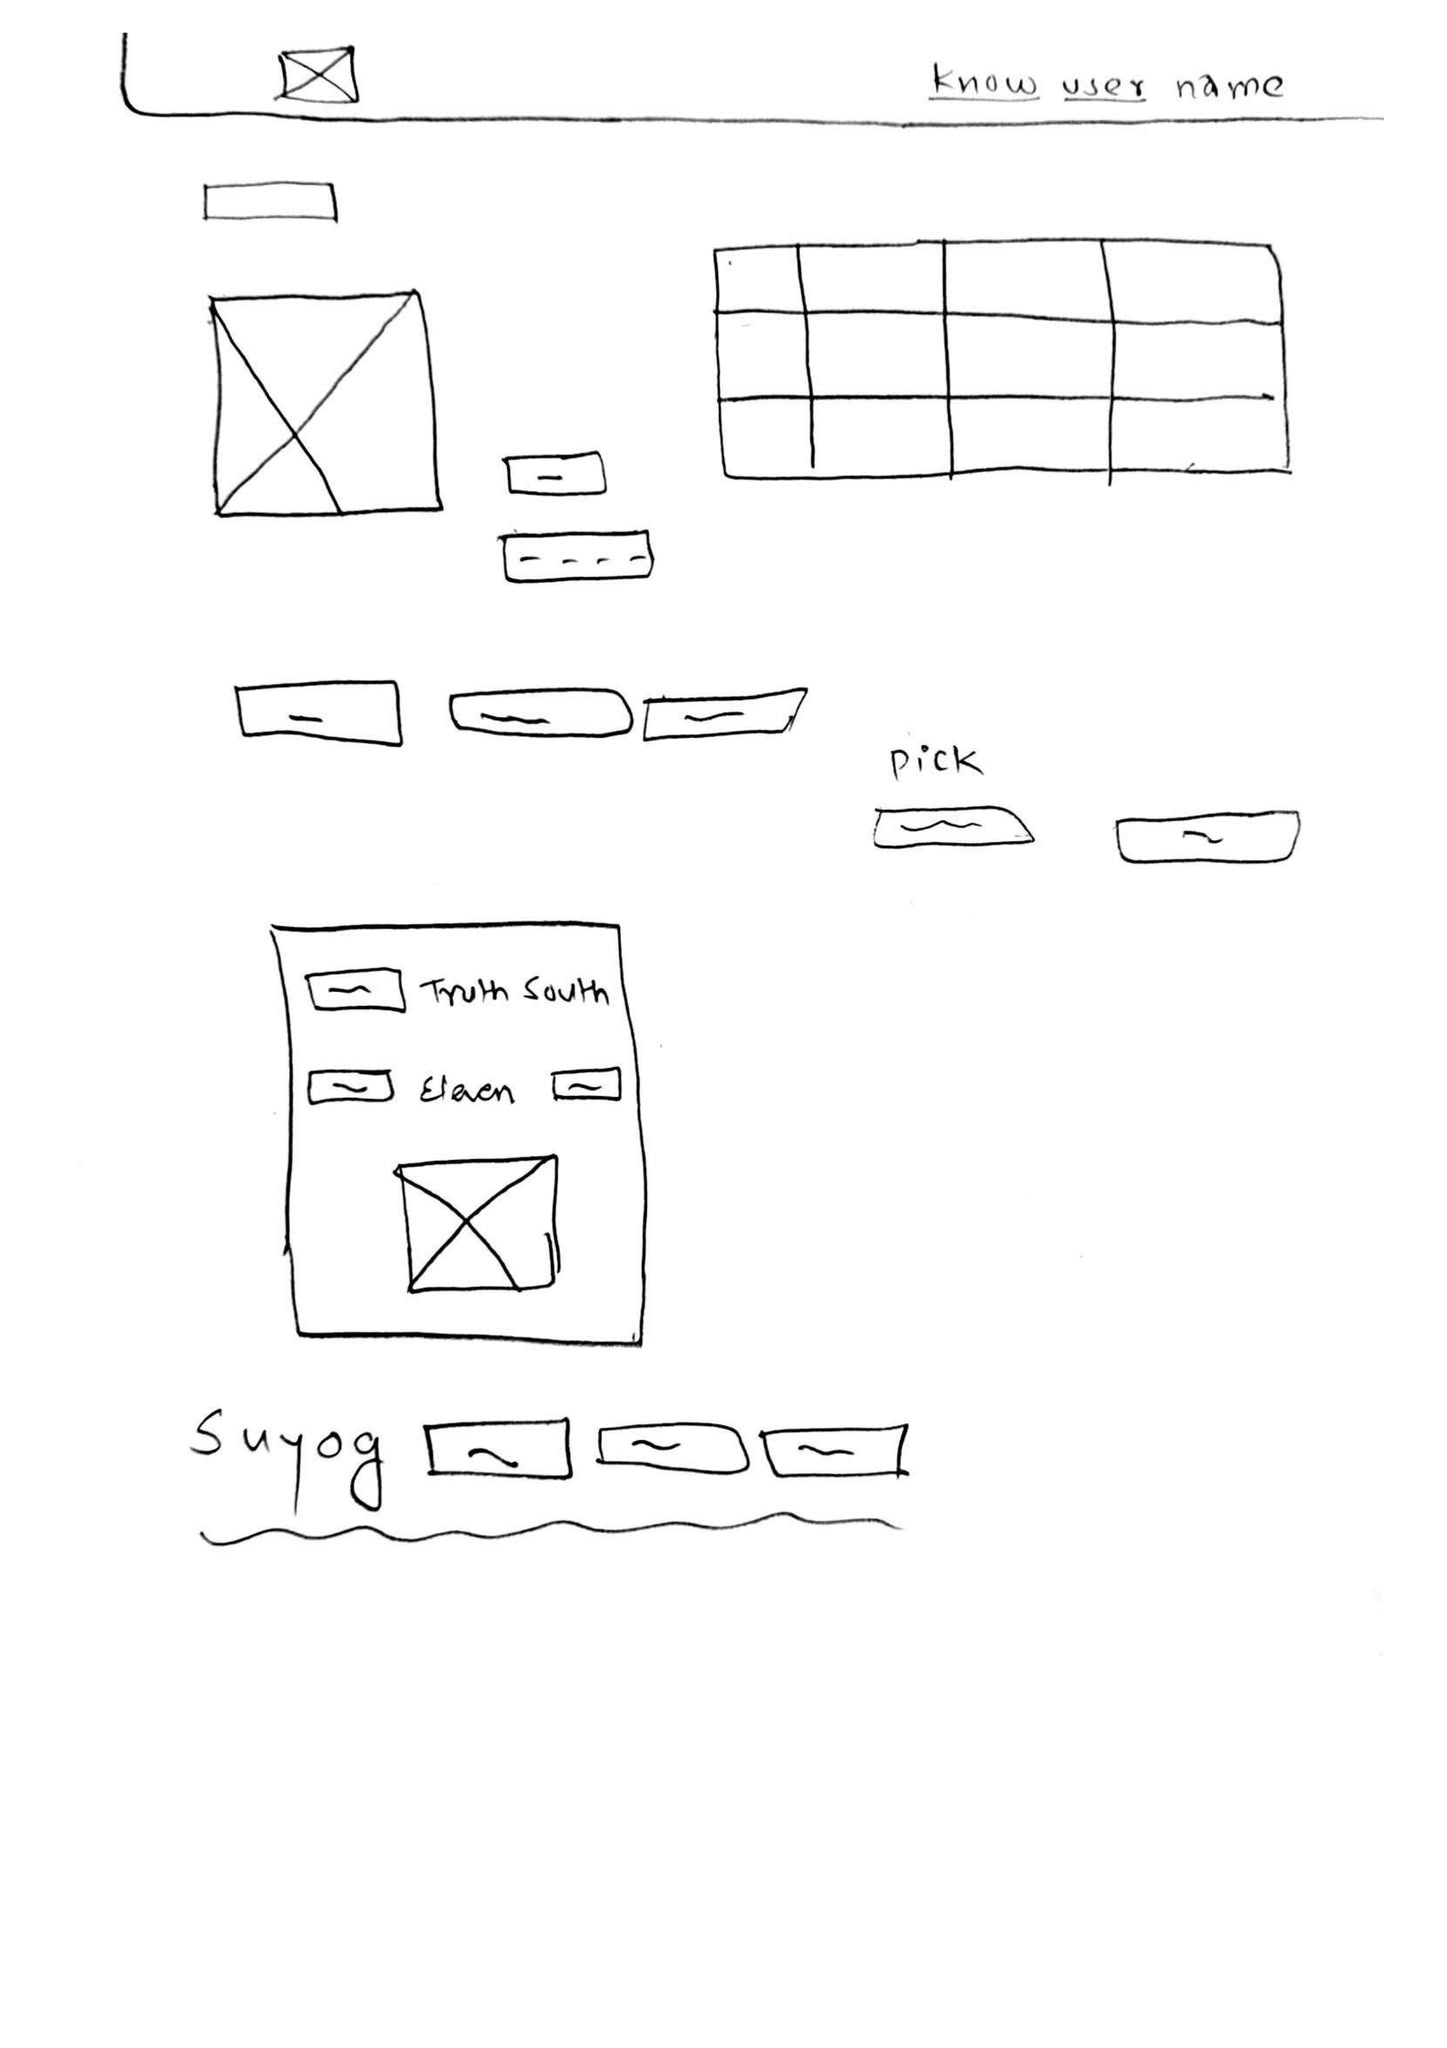
\includegraphics[scale=.2, trim = 0 450 0 0]{images/m2i4.jpg}
    \centering
    \caption{Input Image(ROUGE-L score 0.22)}
    \label{fig:m24}
\end{figure}

\begin{figure}[H]
    \centering
    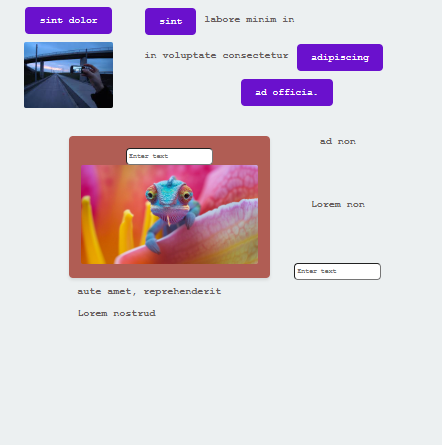
\includegraphics[scale=.6]{images/m2o4.png}
    \caption{Output(ROUGE-L score 0.22)}
    \label{fig:m23}
\end{figure}

\subsubsection{Model 3(Convolutional Encoder with Transformer Decoder)}
\begin{figure}[H]
    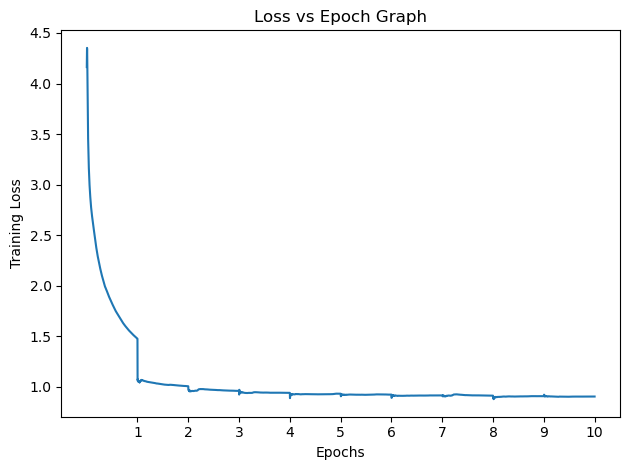
\includegraphics[scale=.8]{images/tl3.png}
    \caption{Training Loss vs Epoch(model 3)}
    \label{fig:tl3}
\end{figure}
\begin{figure}[H]
    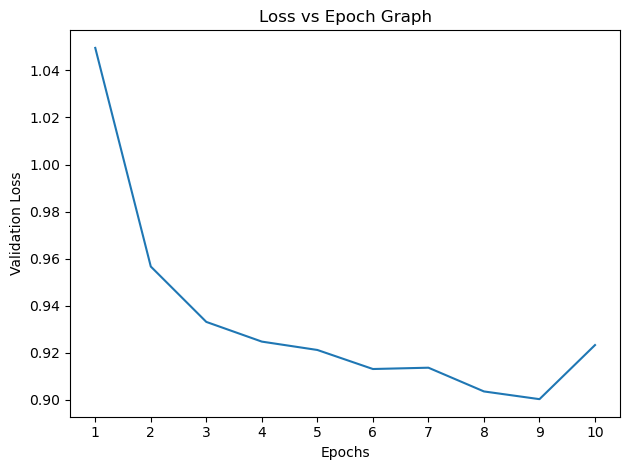
\includegraphics[scale=.8]{images/vl3.png}
    \caption{Validation Loss vs Epoch(model 3)}
    \label{fig:vl3}
\end{figure}
Like other models, the loss of the model was high at the beginning. The loss decreased slowly from 4.2. The training loss doesn’t seem to decrease after 4th epoch. The loss of the training data is in range of about 0.9 after 2nd epoch. The training was stopped after the loss start to increase. The training loss of 0.93 was encountered at the end of 10th epoch. The masked accuracy reached the value of 0.63 for the training data. As the loss of the model didn’t decreased to suitable value the model was not further evalutated.
\subsubsection{Comparison of Model 1 and 2}
Both the model consists of transformer encoder and decoder. In model 2, the patches were extracted from the images were input to the transformer. In model 1, the feature map extracted from the convolutional tokenizer is flattened and provided to the model. The training of the model 2 seems to be slower than the model 1. The model 1 uses learnable positional encoding while model 2 uses sinosudoal positional encoding. The model 1 achieved about 90\% accuracy after 10 epochs while model 2 took more than 20 epochs.By comparing the ROUGE and BLEU score obtained for both models, model 1 outperforms model 2 in terms of metrics. Model 1(4675007) has more trainable params than the model 2 (3210527).
\subsection{Customization}
User can style and customize the layout and visuals of the generated webpage.
\subsubsection{UI}
Here, is the screenshot of the interface which can be used to change the style of the 
generated web page. First, they have to upload the image and then, they can customize the webpage. Here, user can save the desired webpage and they will get html, CSS for that page.

\begin{figure}[H]
    \centering
           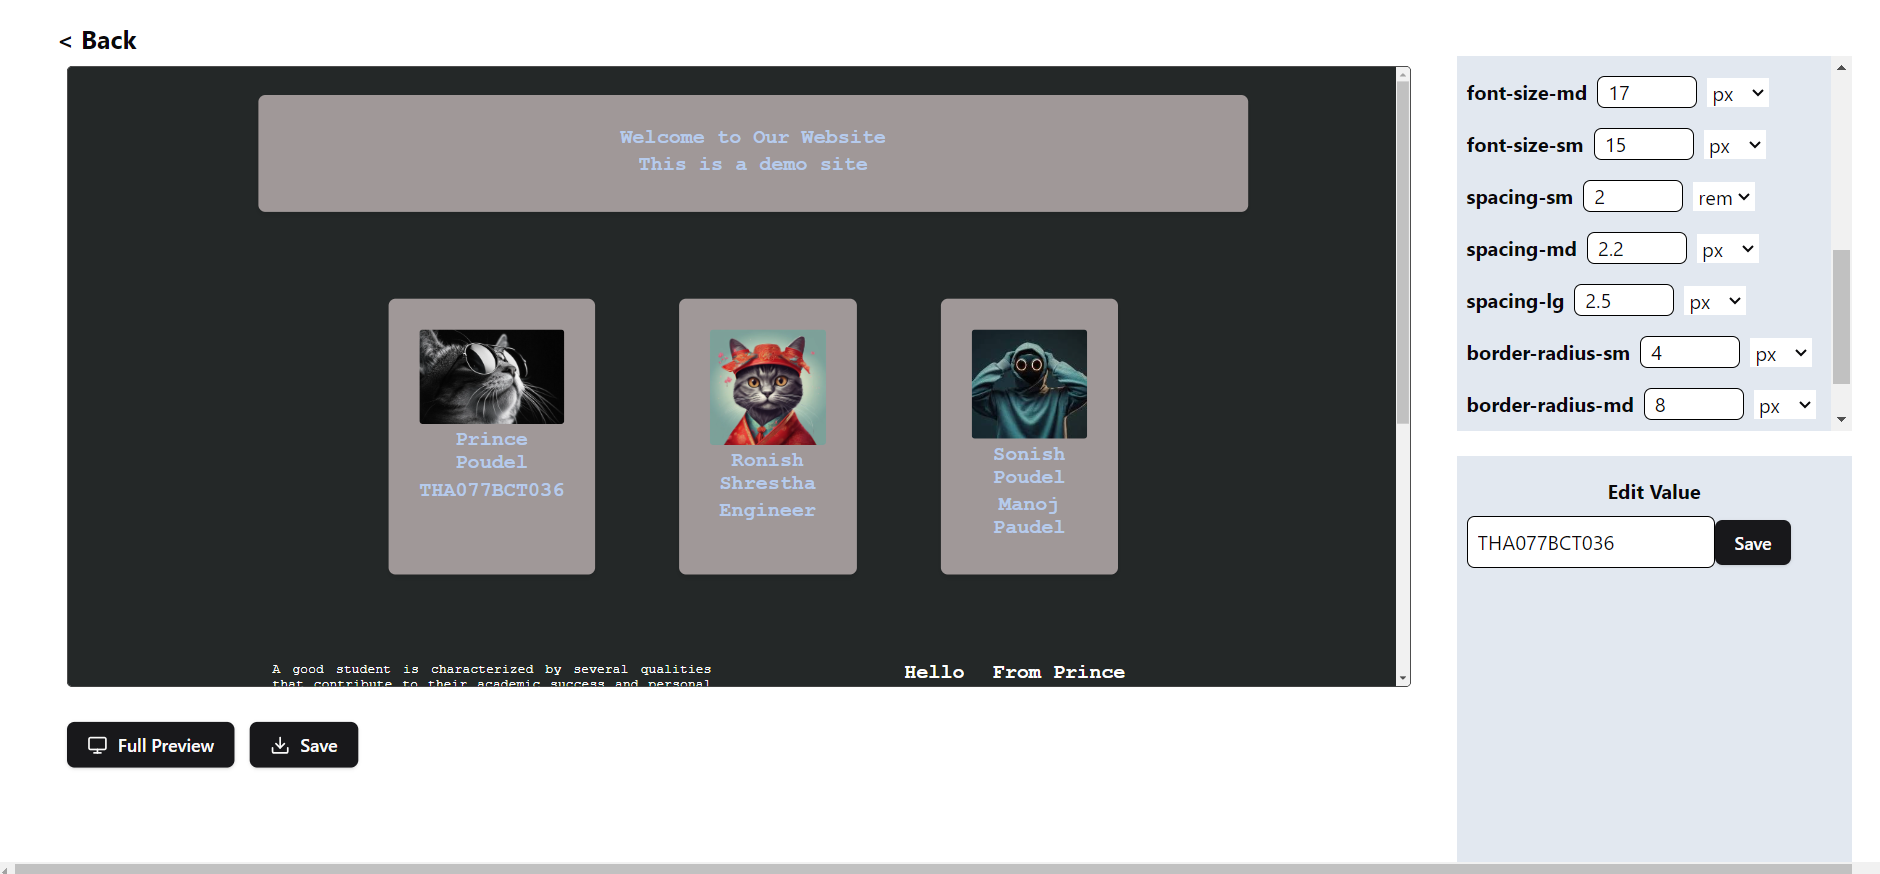
\includegraphics[scale=0.2]{images/user interface.png}
           \caption{User Interface}
           \label{fig:ui}
       \end{figure}
   

\subsubsection{Full Webpage}
This is the webpage that a user can get after customization.

\begin{figure}[H]
    \centering
           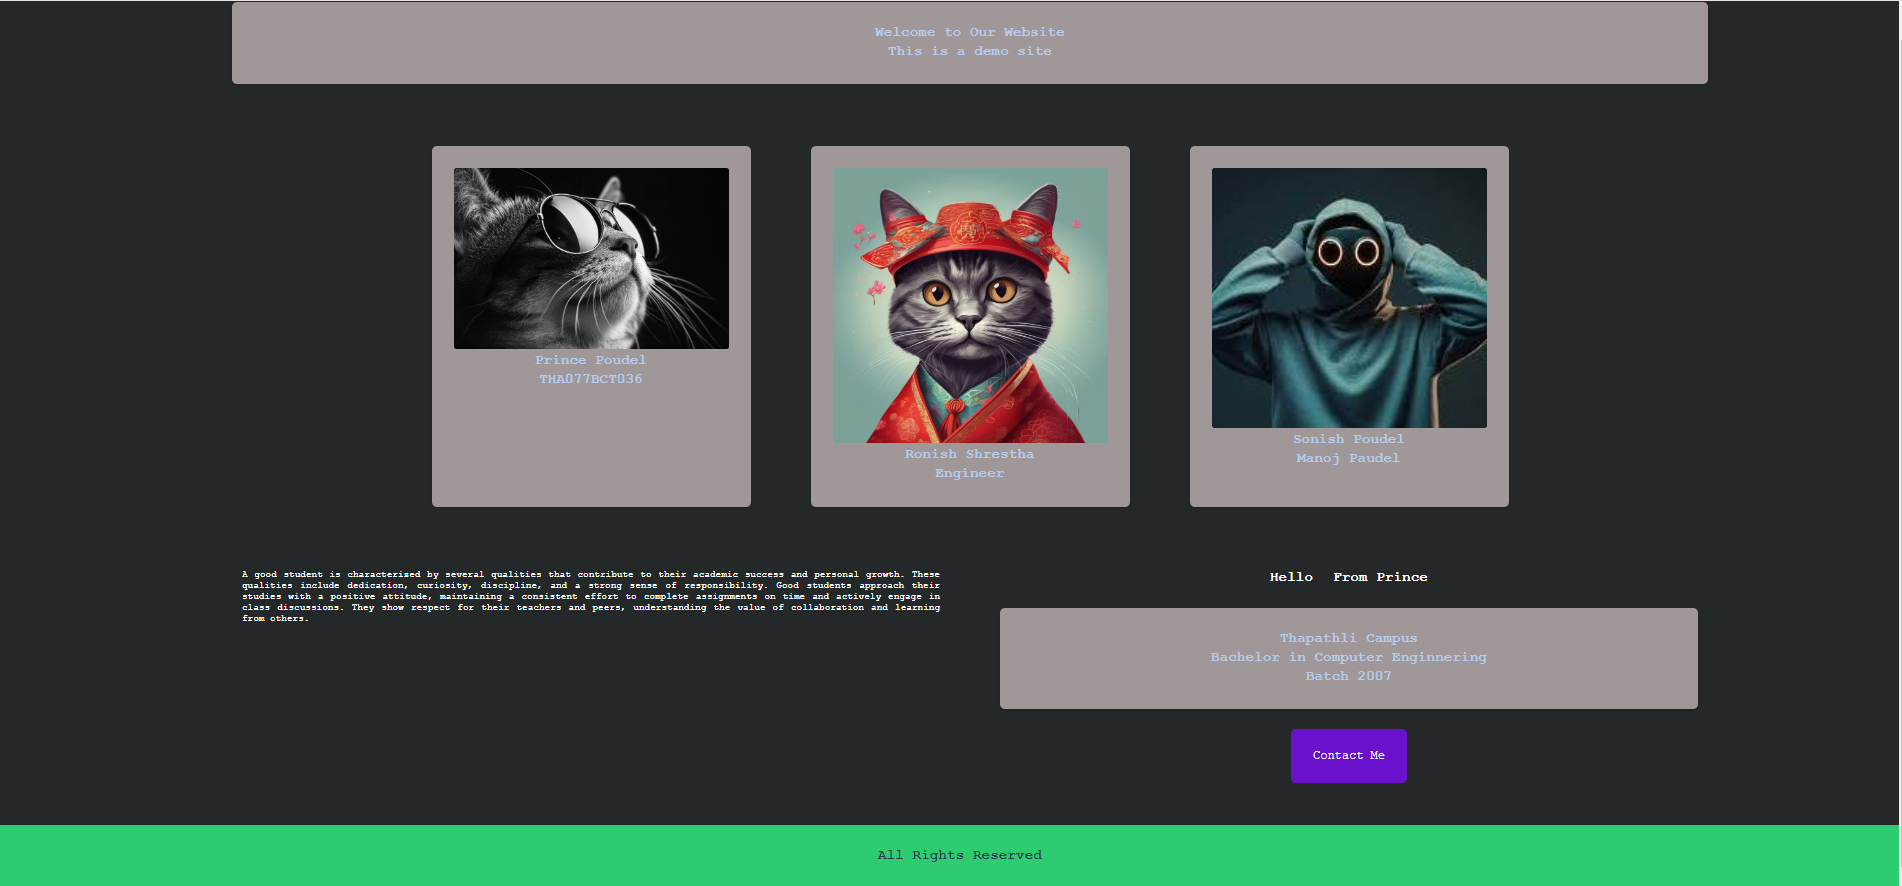
\includegraphics[scale=0.25,trim=230 10 190 10, clip]{images/full webpage.png}
           \caption{Full webpage}
           \label{fig:fullweb}
       \end{figure}


\subsubsection{Customization Options}
Different customization options are available to change the style of webpage. Mainly, user can change the color, text,  
size and text font.  All the options available are given below.

\begin{figure}[H]
    \centering
    \begin{minipage}{0.5\textwidth} % Adjust width to ensure spacing
        \centering
        \vspace{+64pt}
        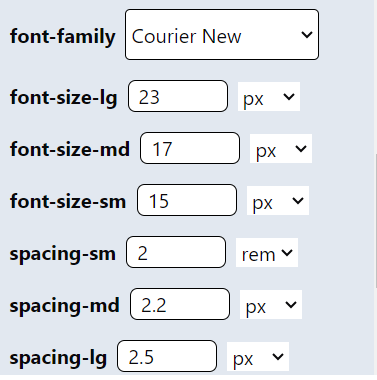
\includegraphics[width=\linewidth]{images/customization 1.png}
        \caption{Font Customization}
        \label{fig:c1}
    \end{minipage}%
    \hfill
    \begin{minipage}{0.5\textwidth}
        \centering
        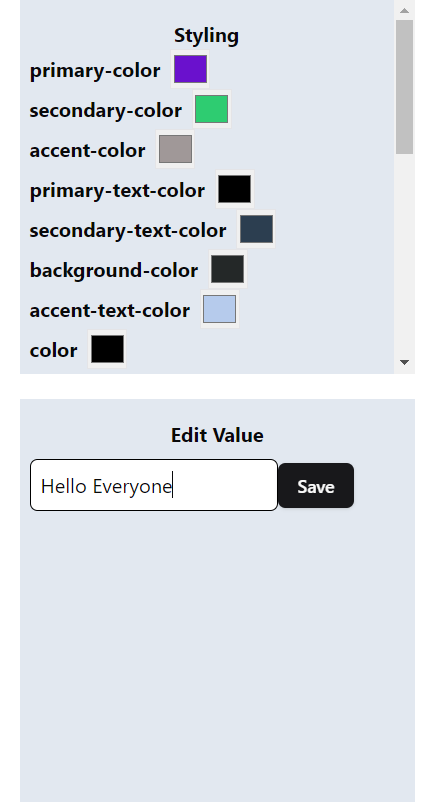
\includegraphics[width=\linewidth, trim=0 250 0 0, clip]{images/customization 2.png}
        \caption{Color Customization}
        \label{fig:c2}
    \end{minipage}
\end{figure}


\subsubsection{JSON file}
This is the sample of the JSON file which have information about the element and the styles. It also carries the changes 
specified by the user through the User interface. Node key helps in carrying the information about the hierarchical structure of the webpage.
 
\begin{verbatim}
    {
        "node": {
          "element": "root",
          "nodes": [
            {
              "element": "header",
              "nodes": [
                {
                  "element": "flex",
                  "nodes": [
                    {
                      "element": "logodiv",
                      "nodes": [
                        {
                          "element": "image",
                          "nodes": [],
                        }
                      ]
                    }
                  ]
                }
              ]
            },
            {
              "element": "container",
              "nodes": [
                {
                  "element": "row",
                  "nodes": [
                    {
                      "element": "div-6",
                      "nodes": [
                        {
                          "element": "image",
                          "nodes": [],
                          "url": "https://..........."
                        }
                      ]
                    }
                  ]
                },
                {
                  "element": "row",
                  "nodes": [
                    {
                      "element": "div-12",
                      "nodes": [
                        {
                          "element": "text",
                          "nodes": [],
                          "text": "About Us"
                        },
                        {
                          "element": "paragraph",
                          "nodes": [],
                          "text": "We …………”
                        }
                      ]
                    }
                  ]
                }
              ]
            }
          ],
          "styles": {
            "accent-color": "#e74c3c",
            "accent-text-color": "black",
            "background-color": "#ecf0f1",
            "border-radius-lg": "12px",
            "border-radius-md": "8px",
            "border-radius-sm": "4px",
            "color": "#1c1717",
            "font-family": "Arial",
            "font-size-lg": "25px",
            "font-size-md": "16px",
            "font-size-sm": "18px",
            "primary-color": "#6a11cd",
            "primary-text-color": "white",
            "secondary-color": "#2ecc71",
            "secondary-text-color": "#2c3e50",
            "spacing-lg": "2rem",
            "spacing-md": "1.5rem",
            "spacing-sm": "1rem"
          }
        }}

\end{verbatim}



\subsubsection{Html File}
This is the sample of the HTML and CSS file which is compiled from the JSON. 
\begin{verbatim}
    <head>
    <meta charset="UTF-8" />
    <meta name="viewport" content="width=device-width, initial-scale=1.0" />
    <title>Generated Page</title>
  </head>
  <body>
    <div id="root" class="root" data-id="110">
      <header class="header" data-id="111">
        <div class="flex" data-id="112">
          <div class="logodiv" data-id="113">
            <img
              src="https://..."
              class="image"
              data-id="114"
            />
          </div>
        </div>
      </header>

      <div class="container" data-id="115">
        <div class="row" data-id="116">
          <div class="div-6" data-id="117">
            <img
              src="https://....
              class="image"
              data-id="118"
            />
          </div>
        </div>
        <div class="row" data-id="119">
          <div class="div-12" data-id="120">
            <div class="text" data-id="121">About Us</div>
            <p class="paragraph" data-id="122">We are</p>
          </div>
        </div>
      </div>
    </div>
  </body>
  
</html>

\end{verbatim}

    \subsection{Sample Generated Datasets}
\textbf{Sample 1}
\begin{verbatim}
    container {
        row {
            div-6 {
                image
                paragraph
            }
            div-6 {
                flex-r {
                    button
                    button
                    text
                }
                carousel
                button
            }
        }
        row {
            div-9 {
                carousel
                input
                text
            }
            div-3 {
                card {
                    image
                    paragraph
                    text-c
                }
                paragraph
            }
        }
        row {
            div-3 {
                card {
                    input
                    input
                }
                input
            }
            div-3 {
                card {
                    paragraph
                    text-c
                }
                button-c
            }
            div-6 {
                paragraph
                button
                text
            }
        }
    }
    footer {
        text-c
    }
    \end{verbatim}
    

\begin{figure}[H]
    \centering
    \begin{minipage}{0.35\textwidth}
        \centering
        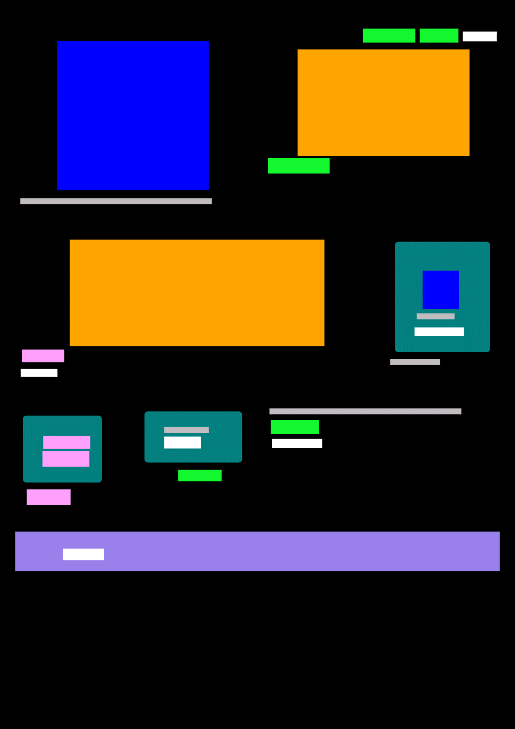
\includegraphics[width=\linewidth]{images/sample1-rendered.png}
        \caption{Rendered HTML}        
        \label{fig:s1}
    \end{minipage}\hfill
    \begin{minipage}{0.35\textwidth}
        \centering
        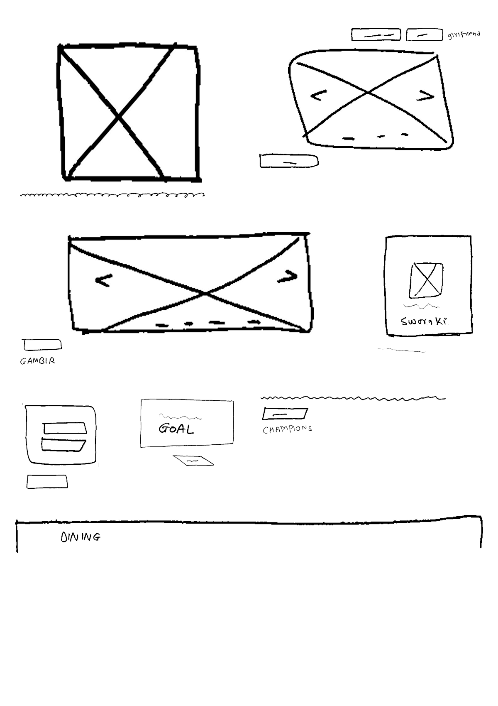
\includegraphics[width=\linewidth]{images/sample1-sketch.png}
        \caption{Sketch}
        \label{fig:s2}
    \end{minipage}
\end{figure}
\vspace{1em} 

    
\textbf{Sample 2}
\begin{verbatim}
    header {
        flex-sb {
            logodiv {
                image
                text
            }
            nav {
                navlink
                navlink
                navlink
                navlink
            }
        }
    }
    container {
        row {
            div-9 {
                input
                flex-sb {
                    button
                    button
                    button
                    text
                }
                table
                button
            }
            div-3 {
                card {
                    paragraph
                    text-c
                    paragraph
                }
                paragraph
            }
        }
        row {
            div-3 {
                button-c
                text
                image
                input
            }
            div-6 {
                paragraph
                carousel
                paragraph
            }
            div-3 {
                text
                button
                image
            }
        }
        row {
            div-3 {
                text-c
                card {
                    button
                    image
                }
                input
            }
        }
    }
    \end{verbatim}    
    \begin{figure}[H]
    \centering
    \begin{minipage}{0.35\textwidth}
        \centering
        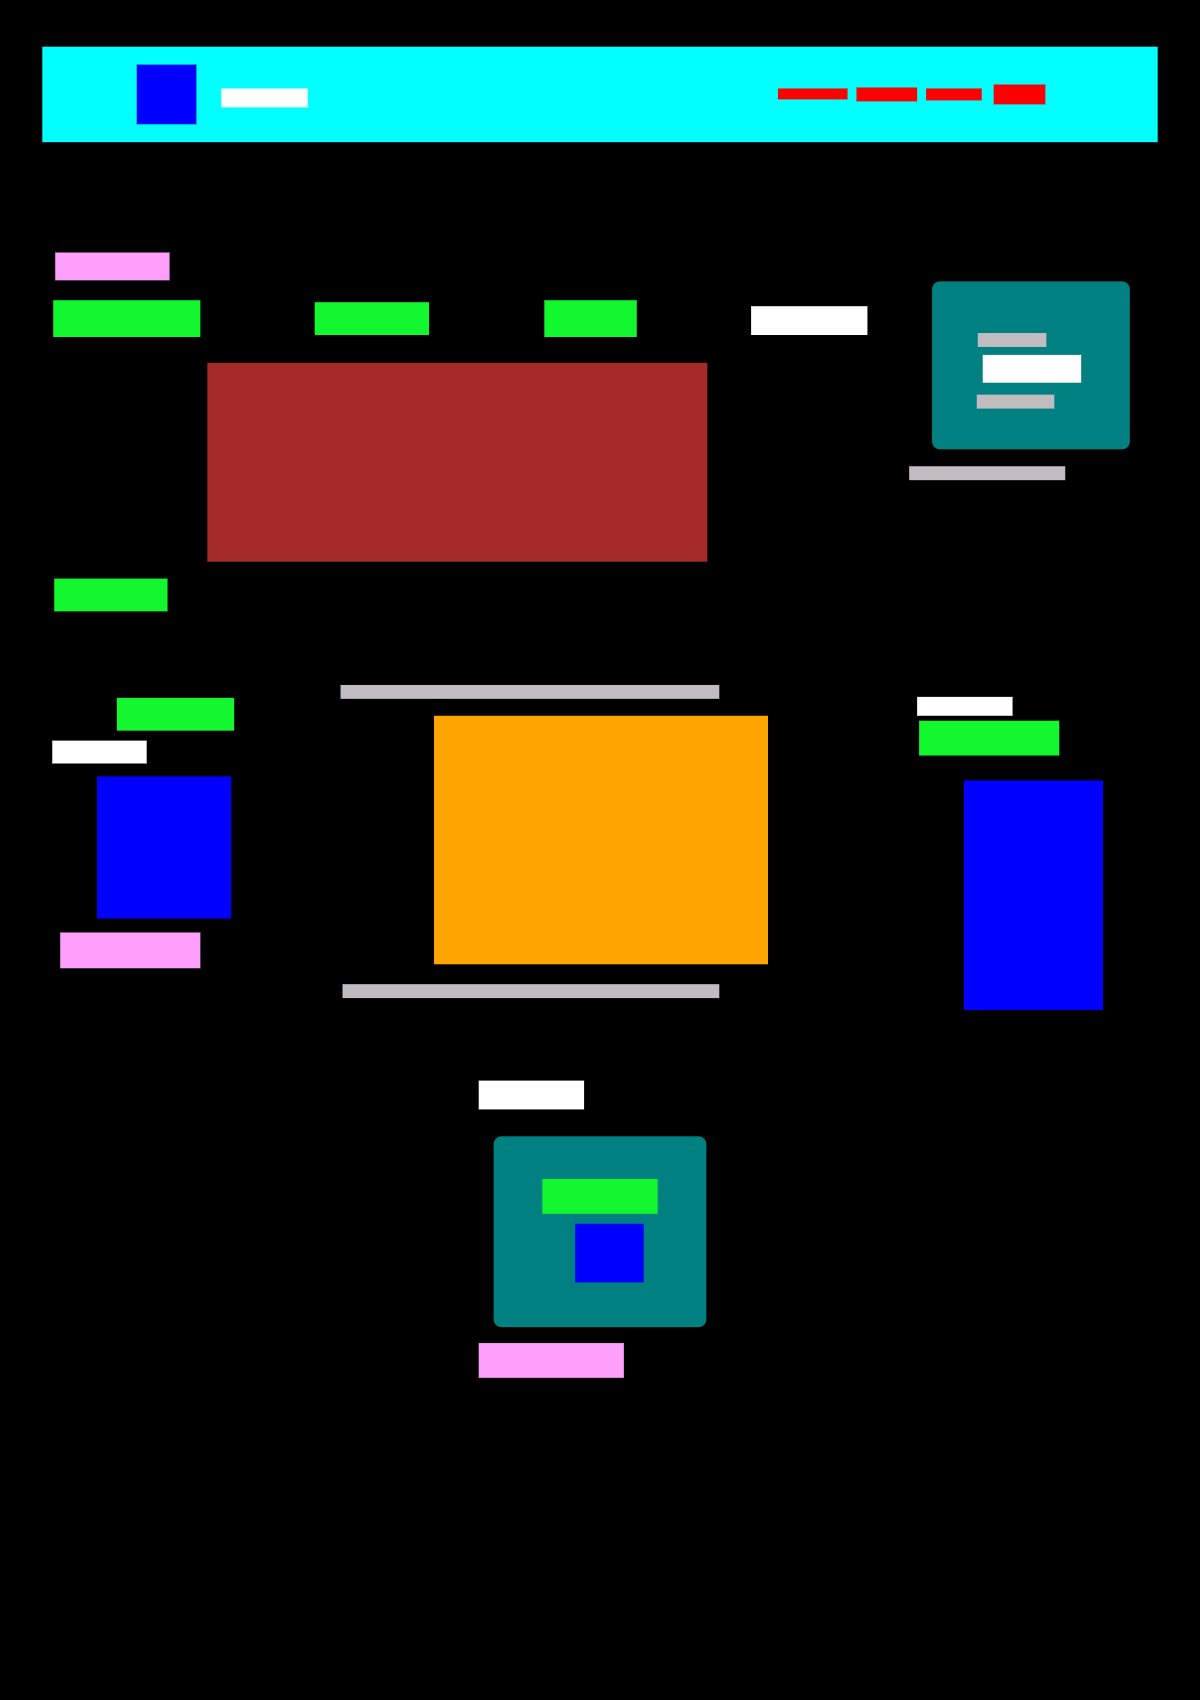
\includegraphics[width=\linewidth]{images/sample2-rendered.png}
        \caption{Rendered HTML}
        \label{fig:s21}
    \end{minipage}\hfill
    \begin{minipage}{0.35\textwidth}
        \centering
        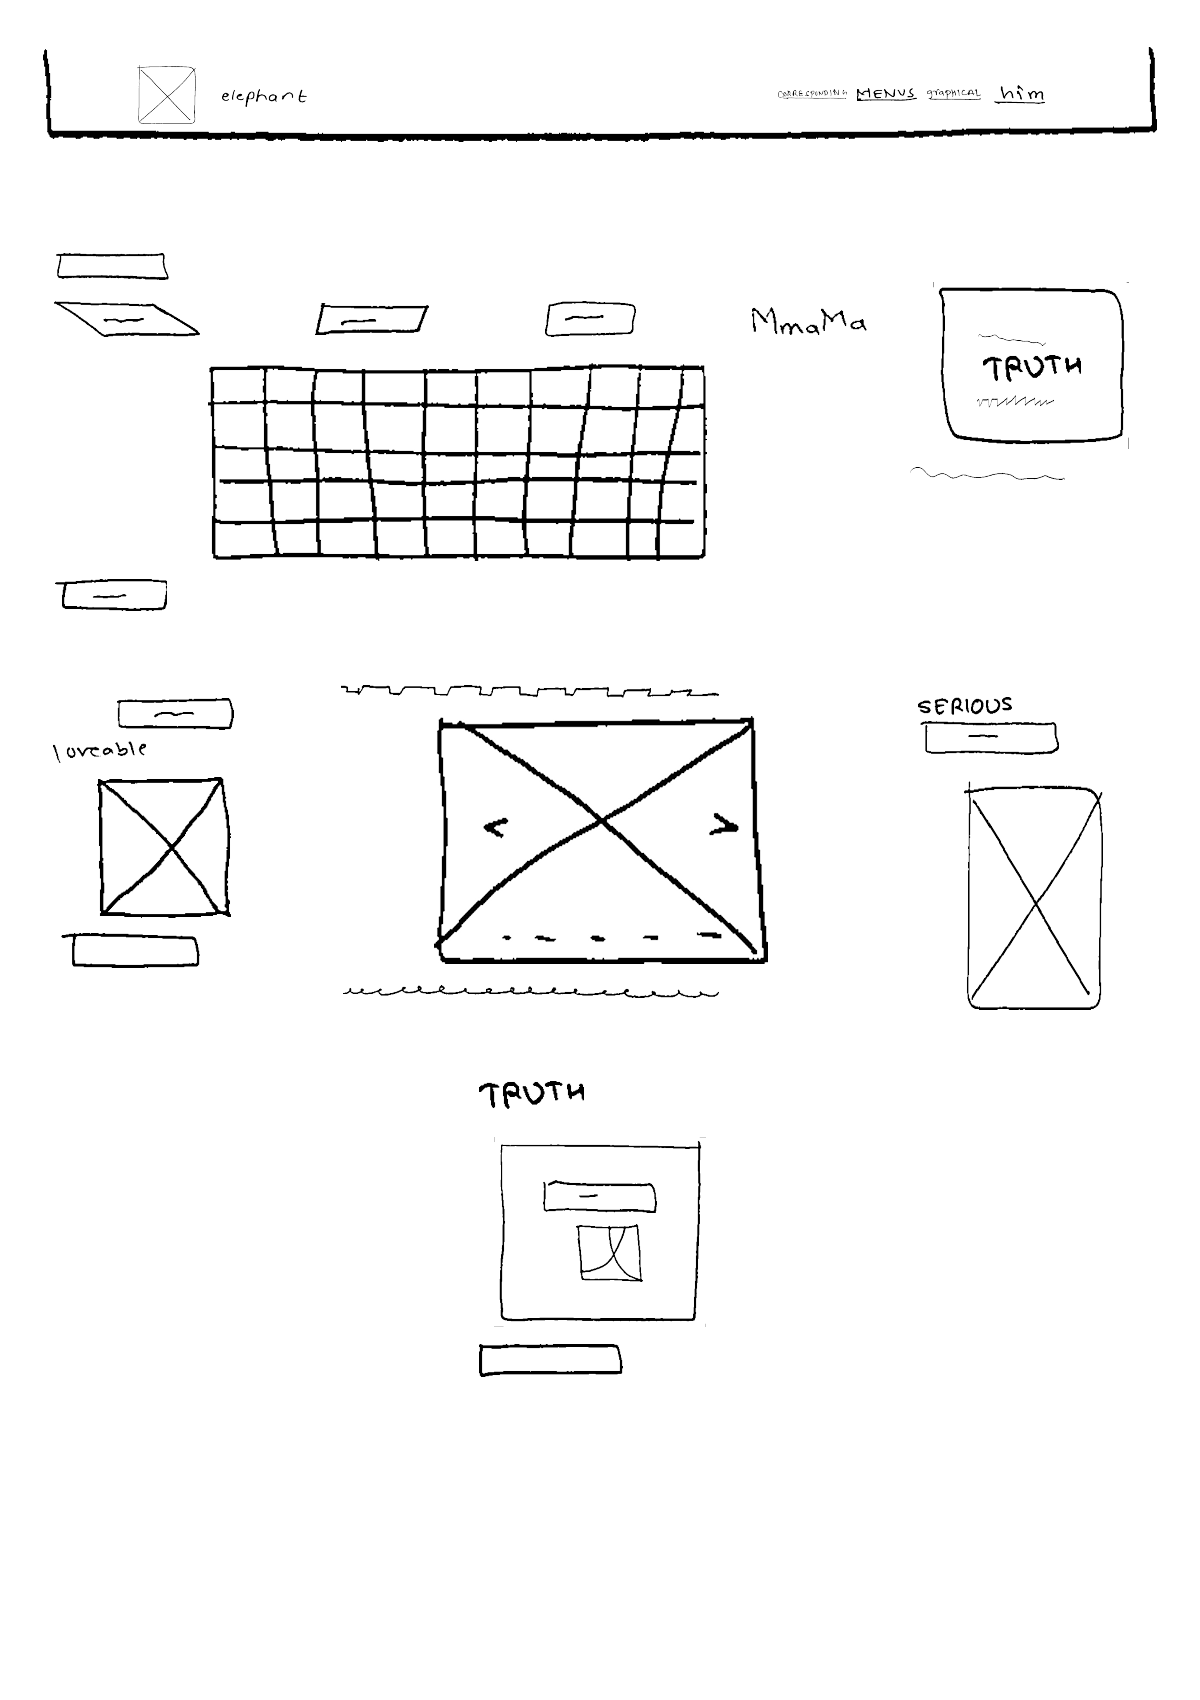
\includegraphics[width=\linewidth]{images/sample2-sketch.png}
        \caption{Sketch}
        \label{fig:s22}
    \end{minipage}
\end{figure}
\vspace{1em} 
    \pagebreak
